\documentclass{standalone}
\usepackage{tikz}
\usetikzlibrary{patterns, positioning}
\usepackage[sfdefault]{ClearSans} %% option 'sfdefault' activates Clear Sans as the default text font
\usepackage[T1]{fontenc}

\begin{document}
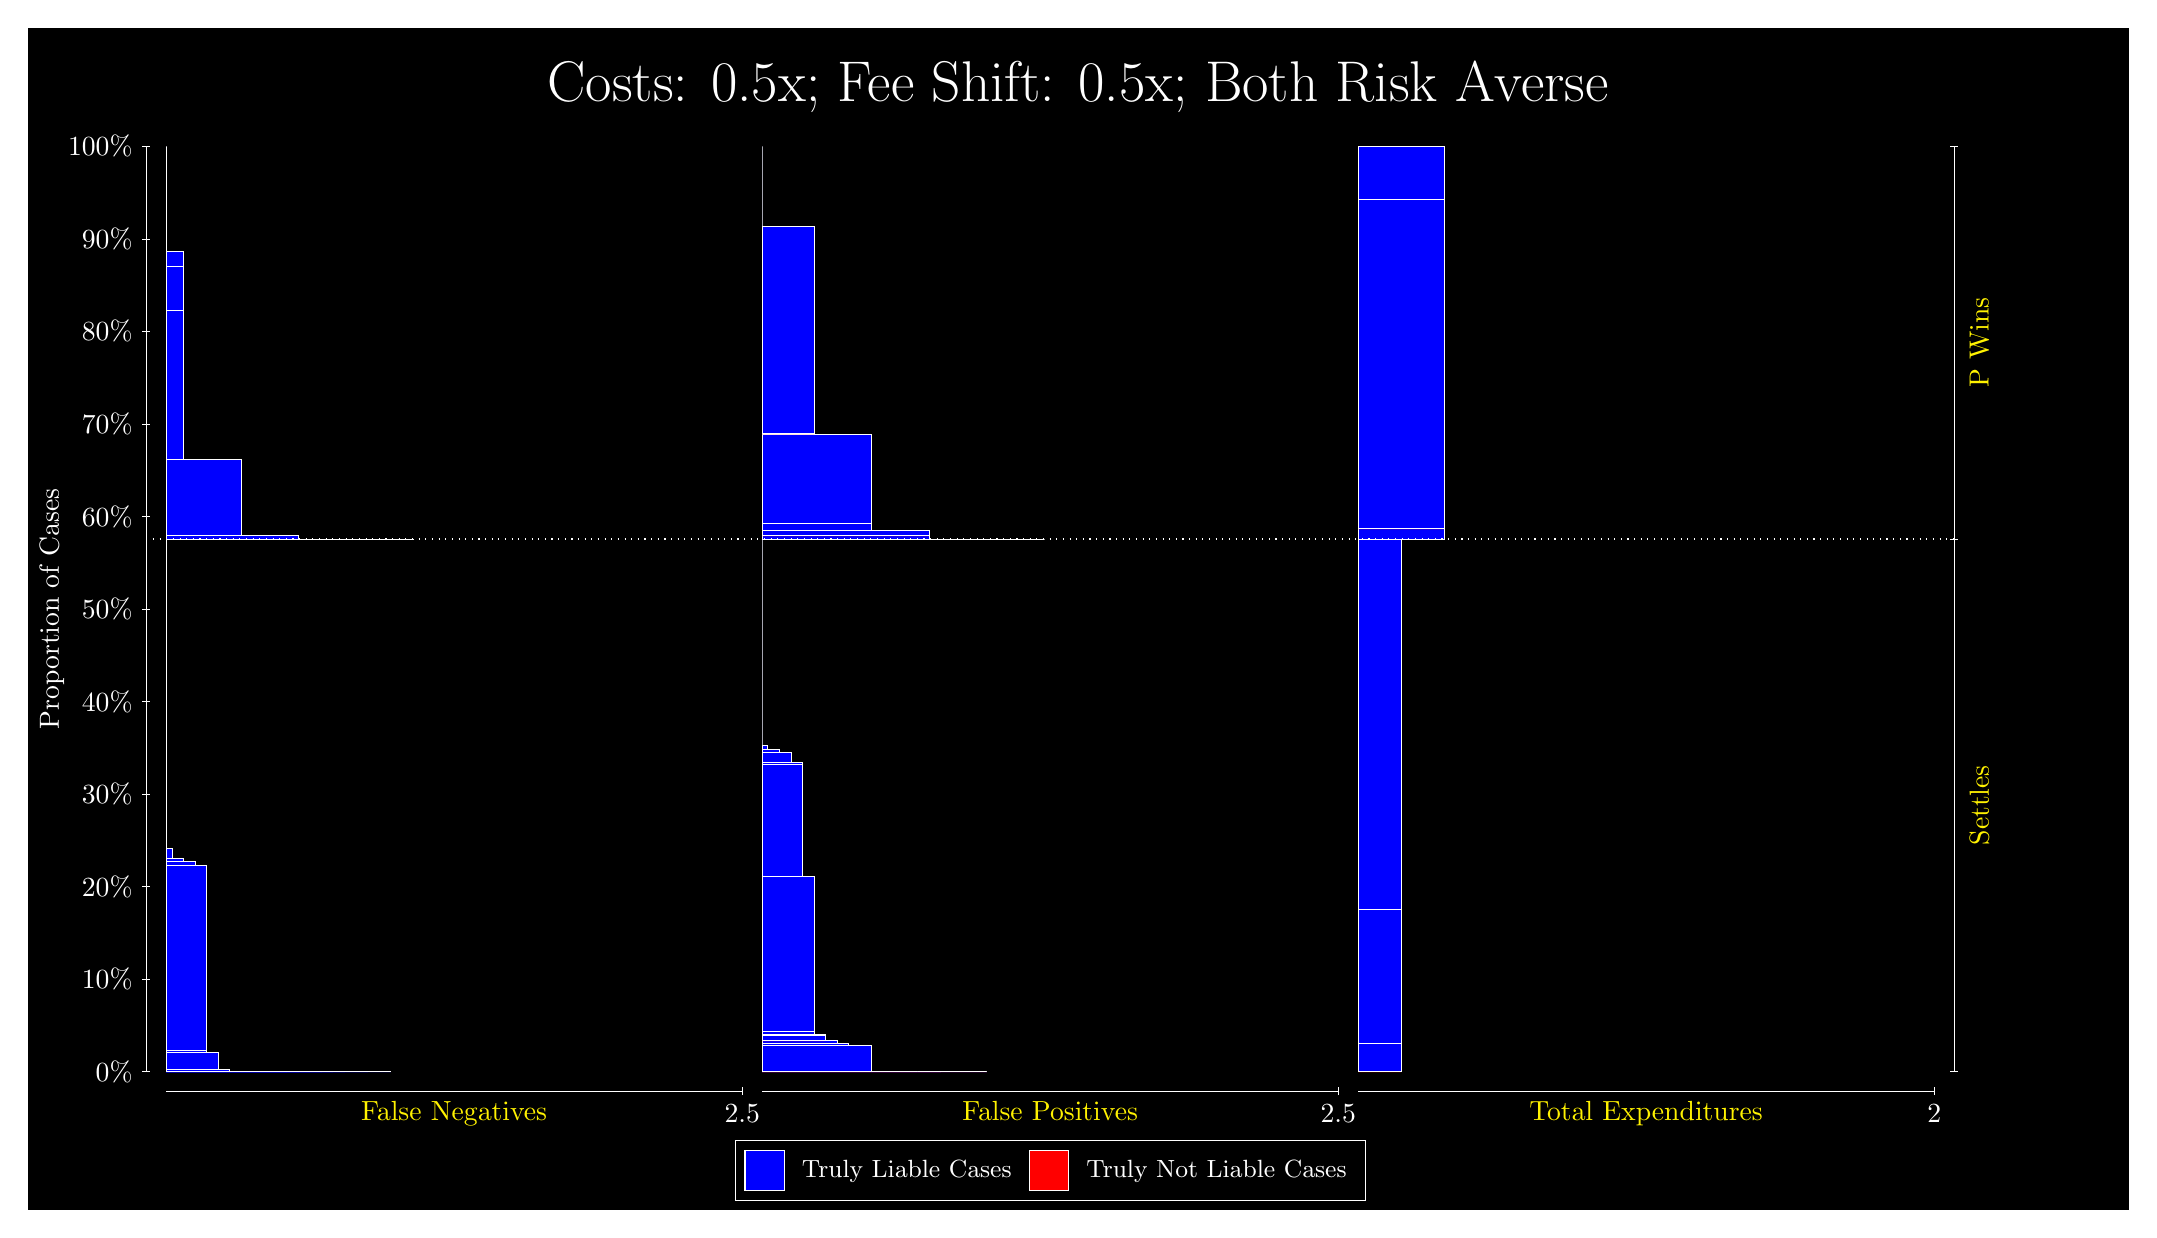
\begin{tikzpicture}
\draw[fill=black] (0,0) rectangle (26.667,15);
\draw[text=white] (0,13.5) rectangle (26.667,15) node[midway] {\huge Costs: 0.5x; Fee Shift: 0.5x; Both Risk Averse};
\draw[white, very thin] (1.5,1.75) -- (1.5,13.5);
\node[rotate=90, text=white, anchor=center] at (0.3, 7.625) {Proportion of Cases};
\draw[white, very thin] (1.45,1.75) -- (1.55,1.75);
\node[text=white, anchor=east] at (1.45, 1.75) {0\%};
\draw[white, very thin] (1.45,2.925) -- (1.55,2.925);
\node[text=white, anchor=east] at (1.45, 2.925) {10\%};
\draw[white, very thin] (1.45,4.1) -- (1.55,4.1);
\node[text=white, anchor=east] at (1.45, 4.1) {20\%};
\draw[white, very thin] (1.45,5.275) -- (1.55,5.275);
\node[text=white, anchor=east] at (1.45, 5.275) {30\%};
\draw[white, very thin] (1.45,6.45) -- (1.55,6.45);
\node[text=white, anchor=east] at (1.45, 6.45) {40\%};
\draw[white, very thin] (1.45,7.625) -- (1.55,7.625);
\node[text=white, anchor=east] at (1.45, 7.625) {50\%};
\draw[white, very thin] (1.45,8.8) -- (1.55,8.8);
\node[text=white, anchor=east] at (1.45, 8.8) {60\%};
\draw[white, very thin] (1.45,9.975) -- (1.55,9.975);
\node[text=white, anchor=east] at (1.45, 9.975) {70\%};
\draw[white, very thin] (1.45,11.15) -- (1.55,11.15);
\node[text=white, anchor=east] at (1.45, 11.15) {80\%};
\draw[white, very thin] (1.45,12.325) -- (1.55,12.325);
\node[text=white, anchor=east] at (1.45, 12.325) {90\%};
\draw[white, very thin] (1.45,13.5) -- (1.55,13.5);
\node[text=white, anchor=east] at (1.45, 13.5) {100\%};

\draw[white, very thin] (24.457,1.75) -- (24.457,13.5);
\draw[white, very thin] (24.407,1.75) -- (24.507,1.75);
\node[anchor=west] at (24.407, 1.75) {};
\draw[white, very thin] (24.407,8.5128) -- (24.507,8.5128);
\node[anchor=west] at (24.407, 8.5128) {};
\draw[white, very thin] (24.407,13.5) -- (24.507,13.5);
\node[anchor=west] at (24.407, 13.5) {};

\draw[white, very thin, fill=blue] (1.75,1.75) rectangle (4.6044,1.75);
\draw[white, very thin, fill=blue] (1.75,1.75) rectangle (4.3116,1.75);
\draw[white, very thin, fill=blue] (1.75,1.75) rectangle (4.0188,1.75);
\draw[white, very thin, fill=blue] (1.75,1.75) rectangle (3.8725,1.75);
\draw[white, very thin, fill=blue] (1.75,1.75) rectangle (3.7261,1.75);
\draw[white, very thin, fill=blue] (1.75,1.75) rectangle (3.5797,1.75);
\draw[white, very thin, fill=blue] (1.75,1.75) rectangle (3.4333,1.75);
\draw[white, very thin, fill=blue] (1.75,1.75) rectangle (3.287,1.75);
\draw[white, very thin, fill=blue] (1.75,1.75) rectangle (3.1406,1.751);
\draw[white, very thin, fill=blue] (1.75,1.751) rectangle (2.9942,1.751);
\draw[white, very thin, fill=blue] (1.75,1.751) rectangle (2.8478,1.7516);
\draw[white, very thin, fill=blue] (1.75,1.7516) rectangle (2.7015,1.7517);
\draw[white, very thin, fill=blue] (1.75,1.7517) rectangle (2.5551,1.7785);
\draw[white, very thin, fill=blue] (1.75,1.7785) rectangle (2.4087,1.9952);
\draw[white, very thin, fill=blue] (1.75,1.9952) rectangle (2.2623,2.0226);
\draw[white, very thin, fill=blue] (1.75,2.0226) rectangle (2.2623,4.3688);
\draw[white, very thin, fill=blue] (1.75,4.3688) rectangle (2.1159,4.4261);
\draw[white, very thin, fill=blue] (1.75,4.4261) rectangle (1.9696,4.4592);
\draw[white, very thin, fill=blue] (1.75,4.4592) rectangle (1.8232,4.589);
\draw[white, very thin, fill=red] (1.75,4.589) rectangle (1.75,4.589);
\draw[white, very thin, fill=blue] (1.75,4.589) rectangle (1.75,8.5128);
\draw[white, very thin, fill=blue] (1.75,8.5128) rectangle (4.8971,8.5128);
\draw[white, very thin, fill=blue] (1.75,8.5128) rectangle (4.1652,8.513);
\draw[white, very thin, fill=blue] (1.75,8.513) rectangle (3.4333,8.5638);
\draw[white, very thin, fill=blue] (1.75,8.5638) rectangle (2.7015,9.5279);
\draw[white, very thin, fill=blue] (1.75,9.5279) rectangle (2.7015,9.529);
\draw[white, very thin, fill=blue] (1.75,9.529) rectangle (1.9696,11.417);
\draw[white, very thin, fill=blue] (1.75,11.417) rectangle (1.9696,11.974);
\draw[white, very thin, fill=blue] (1.75,11.974) rectangle (1.9696,12.166);
\draw[white, very thin, fill=red] (1.75,12.166) rectangle (1.75,12.166);
\draw[white, very thin, fill=blue] (1.75,12.166) rectangle (1.75,13.5);
\draw[white, very thin, fill=red] (9.3189,1.75) rectangle (12.173,1.75);
\draw[white, very thin, fill=blue] (9.3189,1.75) rectangle (12.173,1.75);
\draw[white, very thin, fill=red] (9.3189,1.75) rectangle (11.588,1.75);
\draw[white, very thin, fill=blue] (9.3189,1.75) rectangle (11.588,1.75);
\draw[white, very thin, fill=blue] (9.3189,1.75) rectangle (11.441,1.7512);
\draw[white, very thin, fill=red] (9.3189,1.7512) rectangle (11.295,1.7512);
\draw[white, very thin, fill=blue] (9.3189,1.7512) rectangle (11.295,1.7512);
\draw[white, very thin, fill=red] (9.3189,1.7512) rectangle (11.002,1.7512);
\draw[white, very thin, fill=blue] (9.3189,1.7512) rectangle (11.002,1.7513);
\draw[white, very thin, fill=blue] (9.3189,1.7513) rectangle (10.856,1.7521);
\draw[white, very thin, fill=red] (9.3189,1.7521) rectangle (10.709,1.7521);
\draw[white, very thin, fill=blue] (9.3189,1.7521) rectangle (10.709,1.7524);
\draw[white, very thin, fill=blue] (9.3189,1.7524) rectangle (10.709,2.0844);
\draw[white, very thin, fill=blue] (9.3189,2.0844) rectangle (10.563,2.0852);
\draw[white, very thin, fill=red] (9.3189,2.0852) rectangle (10.417,2.0852);
\draw[white, very thin, fill=blue] (9.3189,2.0852) rectangle (10.417,2.1094);
\draw[white, very thin, fill=blue] (9.3189,2.1094) rectangle (10.27,2.1426);
\draw[white, very thin, fill=red] (9.3189,2.1426) rectangle (10.124,2.1426);
\draw[white, very thin, fill=blue] (9.3189,2.1426) rectangle (10.124,2.2047);
\draw[white, very thin, fill=blue] (9.3189,2.2047) rectangle (10.124,2.2267);
\draw[white, very thin, fill=blue] (9.3189,2.2267) rectangle (9.9776,2.2584);
\draw[white, very thin, fill=blue] (9.3189,2.2584) rectangle (9.9776,4.2333);
\draw[white, very thin, fill=red] (9.3189,4.2333) rectangle (9.8312,4.2333);
\draw[white, very thin, fill=blue] (9.3189,4.2333) rectangle (9.8312,5.6553);
\draw[white, very thin, fill=blue] (9.3189,5.6553) rectangle (9.8312,5.6738);
\draw[white, very thin, fill=blue] (9.3189,5.6738) rectangle (9.6848,5.8036);
\draw[white, very thin, fill=blue] (9.3189,5.8036) rectangle (9.5384,5.8367);
\draw[white, very thin, fill=blue] (9.3189,5.8367) rectangle (9.3921,5.893);
\draw[white, very thin, fill=blue] (9.3189,5.893) rectangle (9.3921,5.894);
\draw[white, very thin, fill=blue] (9.3189,5.894) rectangle (9.3189,8.5128);
\draw[white, very thin, fill=red] (9.3189,8.5128) rectangle (12.905,8.5128);
\draw[white, very thin, fill=blue] (9.3189,8.5128) rectangle (12.905,8.5128);
\draw[white, very thin, fill=blue] (9.3189,8.5128) rectangle (12.173,8.5136);
\draw[white, very thin, fill=red] (9.3189,8.5136) rectangle (12.173,8.5136);
\draw[white, very thin, fill=blue] (9.3189,8.5136) rectangle (12.173,8.5141);
\draw[white, very thin, fill=blue] (9.3189,8.5141) rectangle (11.441,8.5563);
\draw[white, very thin, fill=red] (9.3189,8.5563) rectangle (11.441,8.5563);
\draw[white, very thin, fill=blue] (9.3189,8.5563) rectangle (11.441,8.6244);
\draw[white, very thin, fill=blue] (9.3189,8.6244) rectangle (10.709,8.7121);
\draw[white, very thin, fill=red] (9.3189,8.7121) rectangle (10.709,8.7121);
\draw[white, very thin, fill=blue] (9.3189,8.7121) rectangle (10.709,9.847);
\draw[white, very thin, fill=blue] (9.3189,9.847) rectangle (9.9776,9.8495);
\draw[white, very thin, fill=red] (9.3189,9.8495) rectangle (9.9776,9.8495);
\draw[white, very thin, fill=blue] (9.3189,9.8495) rectangle (9.9776,12.484);
\draw[white, very thin, fill=blue] (9.3189,12.484) rectangle (9.3189,13.5);
\draw[white, very thin, fill=red] (16.888,1.75) rectangle (17.437,1.75);
\draw[white, very thin, fill=blue] (16.888,1.75) rectangle (17.437,2.1095);
\draw[white, very thin, fill=red] (16.888,2.1095) rectangle (17.437,2.1095);
\draw[white, very thin, fill=blue] (16.888,2.1095) rectangle (17.437,3.8147);
\draw[white, very thin, fill=red] (16.888,3.8147) rectangle (17.437,3.8147);
\draw[white, very thin, fill=blue] (16.888,3.8147) rectangle (17.437,8.5128);
\draw[white, very thin, fill=red] (16.888,8.5128) rectangle (17.986,8.5128);
\draw[white, very thin, fill=blue] (16.888,8.5128) rectangle (17.986,8.646);
\draw[white, very thin, fill=red] (16.888,8.646) rectangle (17.986,8.646);
\draw[white, very thin, fill=blue] (16.888,8.646) rectangle (17.986,12.832);
\draw[white, very thin, fill=red] (16.888,12.832) rectangle (17.986,12.832);
\draw[white, very thin, fill=blue] (16.888,12.832) rectangle (17.986,13.5);
\draw[white, dotted] (1.5,8.5128) -- (24.457,8.5128);
\draw[white, very thin] (1.75,1.5) -- (9.0689,1.5);
\node[text=yellow, anchor=north] at (5.4094, 1.5) {False Negatives};
\draw[white, very thin] (9.0689,1.45) -- (9.0689,1.55);
\node[text=white, anchor=north] at (9.0689, 1.45) {2.5};

\draw[white, very thin] (9.3189,1.5) -- (16.638,1.5);
\node[text=yellow, anchor=north] at (12.978, 1.5) {False Positives};
\draw[white, very thin] (16.638,1.45) -- (16.638,1.55);
\node[text=white, anchor=north] at (16.638, 1.45) {2.5};

\draw[white, very thin] (16.888,1.5) -- (24.207,1.5);
\node[text=yellow, anchor=north] at (20.547, 1.5) {Total Expenditures};
\draw[white, very thin] (24.207,1.45) -- (24.207,1.55);
\node[text=white, anchor=north] at (24.207, 1.45) {2};

\node[text=yellow, centered, rotate=90] at (24.777, 5.1314) {Settles};
\node[text=yellow, centered, rotate=90] at (24.777, 11.006) {P Wins};

\draw (12.978300999999998,1.5) node[draw=none] (baseCoordinate) {};
\begin{scope}[align=center]
        \matrix[scale=0.5, draw=white, below=0.5cm of baseCoordinate, nodes={draw}, column sep=0.1cm]{
            \node[rectangle, draw, minimum width=0.5cm, minimum height=0.5cm, fill=blue] {}; &
            \node[draw=none, font=\small, text=white] (B) {Truly Liable Cases}; &
            \node[rectangle, draw, minimum width=0.5cm, minimum height=0.5cm, fill=red] {}; &
            \node[draw=none, font=\small, text=white] (B) {Truly Not Liable Cases}; \\
            };
\end{scope}

\end{tikzpicture}
\end{document}